% -----------------------------------------------
% Template for ISMIR Papers
% 2021 version, based on previous ISMIR templates

% Requirements :
% * 6+n page length maximum
% * 10MB maximum file size
% * Copyright note must appear in the bottom left corner of first page
% * Clearer statement about citing own work in anonymized submission
% (see conference website for additional details)
% -----------------------------------------------

\documentclass{article}
\usepackage[T1]{fontenc} % add special characters (e.g., umlaute)
\usepackage[utf8]{inputenc} % set utf-8 as default input encoding
\usepackage{ismir,amsmath,url,cite}
\usepackage{graphicx}
\usepackage{color}
\usepackage{amsmath}
\usepackage{amssymb}
\usepackage{svg}
\usepackage{subcaption}
\captionsetup{compatibility=false}


\graphicspath{{donnees}}

\usepackage{lineno}
\linenumbers

% Title. Please use IEEE-compliant title case when specifying the title here,
% as it has implications for the copyright notice
% ------

%\title{A\lowercase{udio} n\lowercase{etworks} h\lowercase{acking}: n\lowercase{ovelty} s\lowercase{earch} t\lowercase{hrough} a\lowercase{ctive} d\lowercase{ivergence} \\ ATIAM 2022 - ML P\lowercase{roject}}
\title{Audio networks hacking:\\ novelty search through active divergence}

\renewcommand{\permission}{ }

% Note: Please do NOT use \thanks or a \footnote in any of the author markup

% Single address
% To use with only one author or several with the same address
% ---------------
%\oneauthor
% {Names should be omitted for double-blind reviewing}
% {Affiliations should be omitted for double-blind reviewing}

% Two addresses
% --------------
%\twoauthors
%  {First author} {School \\ Department}
%  {Second author} {Company \\ Address}

% Three addresses
% --------------\input{ISMIR2021_paper.tex}

\fourauthors
  {Zhuomin LIU} {{\tt zhuomin.liu@ircam.fr}}
  {Pierre THIEL} {{\tt pierre.thiel@ircam.fr}}
  {Christophe WEIS} {{\tt christophe.weis@ircam.fr}}
  {Roy YAKOOB AL HAKEEM} {{\tt roy.yakoob@ircam.fr}}


%\author{
%  Pierre THIEL,
%  Christophe WEIS,
%  Roy YAKOOB AL HAKEEM,
%  Zhuomin LIU
%}

% Four or more addresses
% OR alternative format for large number of co-authors
% ------------
%\multauthor
%{First author$^1$ \hspace{1cm} Second author$^1$ \hspace{1cm} Third author$^2$} { \bfseries{Fourth author$^3$ \hspace{1cm} Fifth author$^2$ \hspace{1cm} Sixth author$^1$}\\
%  $^1$ Department of Computer Science, University , Country\\
%$^2$ International Laboratories, City, Country\\
%$^3$  Company, Address\\
%{\tt\small CorrespondenceAuthor@ismir.edu, PossibleOtherAuthor@ismir.edu}
%}

% For the author list in the Creative Common license, please enter author names. 
% Please abbreviate the first names of authors and add 'and' between the second to last and last authors.

\def\authorname{L. Zhuomin, P. Thiel, C. Weis, and R. Yakoob Al Hakeem}

% Optional: To use hyperref, uncomment the following.
%\usepackage[bookmarks=false,pdfauthor={\authorname},pdfsubject={\papersubject},hidelinks]{hyperref}
% Mind the bookmarks=false option; bookmarks are incompatible with ismir.sty.

\sloppy % please retain sloppy command for improved formatting

\begin{document}

%
\maketitle
%

%+ Bien analyser les résultats.
%Réduction des dimensions par \textbf{ICA} (gardes les axes perpandiculaires), UMAP, etc.
%Contributions

%reducing the dimensionality of the data we are using, as well as the learning time for your cases. Another very good thing is the compactness and speed in coding using backpropagation. Autoencoders can be great for feature extraction.



\begin{abstract}
%The abstract should be placed at the top left column and should contain about 150-200 words.
Variational auto-encoders are probabilistic generative neural networks based on joint training of an encoder and a decoder, respectively learning low-dimensional latent representations and reconstructing the original data by sampling in the latent space.
In this work, we present our implementation of a VAE and the results obtained by training it on the MNIST database.
Then, aiming at exploring the capacities of VAEs to generate novel objects, we consider different recent approaches of corrupting the model and exploring the latent space that can be referred to by the notion of \emph{active divergence}. We finally illustrate our results obtained by implementing procedures proposed by recent literature.
\end{abstract}



%%%%%%%%%%%%%%%%%%%%%%%%%%%%%%%%%%%%%%%%%%%%%%%%%%%%%%%%%%%%

\section{Introduction}
While classical metrics for generative networks are often measured in terms of quality of generation and fidelity concerning well-known types, recent studies have been focused on the ability of generative models to create \emph{out-of-distribution} data, that is, data that is outside of the task it was trained for.
The qualitative value of novelty has been subject to many aesthetic studies.
They have, for instance, been discussed in the context of computational generative art concerning a trade-off between an exterior user assessment of the value of newly generated objects and implicit system-generated criteria for novelty. 

In this work, we first recall basic concepts and formalisations on \emph{Generative Adversarial Networks} and \emph{Variational Auto-Encoders}. We then investigate recent works on the capacities of generative networks to allow novelty search. Thus, we present three approaches in the field of \emph{active divergence}. \\
We then discuss our experimental setup and results after training our models on the BinaryMNIST and MNIST data sets.
We address the implications of applying corrupting operations, for instance by manipulating our model's weights.
Lastly, we approach a method to generate novelties by exploring latent space representations by an iterative implementation of the auto-encoder starting from random images.


%%%%%%%%%%%%%%%%%%%%%%%%%%%%%%%%%%%%%%%%%%%%%%%%%%%%%%%%%%%%

\section{Related Work}
\label{sec:related_work}

\subsection{Generative Adversarial Networks}
\label{subsec:gan}

The GAN 
\cite{goodfellowGenerativeAdversarialNetworks2020} architecture is built upon an idea that 
two agents with opposite goals can
be made to improve when set against each other in a competitive unsupervised task.
The first agent is a generative network, called \emph{generator},
the second is a classifier, called \emph{discriminator}.
The two agents are trained successively in a loop from a given data set.
The discriminator learns to identify images taken from the original data set and those created by the generator.
The generator then fools the discriminator by creating images closer to the data set.
Neither network should become 
so good as to hinder the improvement of the other and tip the balance of the overall model.
By careful joint training of the two,
both the generator and the discriminator should improve at their respective task.

The GAN can also be interpreted from a game theory standpoint as a game with the 
generator and discriminator being the two players.

In its original formulation, the generator network $G$ takes a latent vector $z$ sampled 
from a set prior distribution $p(z)$, usually uniform or multivariate Gaussian.
As such, $z$ is generally just noise and the relationship between its value and 
that of $\hat{x}$ cannot be readily understood. Thus, there is no way to choose the desired 
features of data generated: for instance, it is not possible to give a reference 
data point $x$ for the generator to try and imitate.

\subsection{Auto-Encoders}
\label{subsec:ae}


In this setting, $x$ is a random variable supposed to be in some way generated from an unobserved $z$,
following an intractable parametric prior distribution $p(z)$.
$z$ is a continuous random variable interpreted as a \emph{latent representation} of $x$.

The auto-encoder is defined as the combination of two networks:
an encoding agent, the \emph{encoder}, aiming at capturing the \emph{posterior} $p(z|x)$, 
and a decoding agent, the \emph{decoder}, computing the \emph{likelihood} of $x$ under $z$ $p(x|z)$.
The generated output $\hat{x}$ is then:
\begin{equation}
    \hat{x} = D \circ E(x) = D(z),
    \label{eq:ae_form}
\end{equation}
where $E$ and $D$ are respectively the \emph{encoder} and \emph{decoder}.
As there is no source of randomness, the classic auto-encoder is deterministic
and cannot model the distribution $p(x)$.
As a result, the latent space has no guarantee to
model recognisable features of the data space.

\subsection{Variational Auto-Encoders}
\label{subsec:vae}

The Variational Auto-Encoder (VAE) is an extension of the well-known auto-encoder
architecture designed to address the issues arising with the deterministic formulation.
In the case of the VAE, the prior, likelihood and
posteriors are assumed to be parametric distributions
of an unknown and unobserved $\theta$.

The \emph{evidence} $p_{\theta}(x)$ can be marginalised thus:
\begin{equation}
    \centering
    p_\theta(x) = \int p_\theta(x|z) \; p_\theta(z) \,dz.
    \label{eq:vae_marg}
\end{equation}
In other words, the data point $x$ can be generated from the prior and the \emph{likelihood} $p_\theta(x|z)$.
Because the real posterior is intractable, an \emph{approximate posterior}
$q_\phi(z|x)$ is defined such that its parameters $\phi$ are learnt jointly with $\theta$.
We use the approximation to find an appropriate lower bound for
the evidence $p_{\theta}(x)$ with regards to $\theta$.

From \ref{eq:vae_marg} we can deduce the
Evidence Lower Bound (ELBO) $\mathcal{L}$ formulation \cite{kingmaAutoEncodingVariationalBayes2014a}:
\begin{equation}
    \centering
    \begin{aligned}
    \log p_\theta(x^{(i)}) & \geq \mathcal{L}(\theta, \phi; x^{(i)}),
    \\
    \mathcal{L}(\theta, \phi; x^{(i)}) &=            
    \mathbb{E}_{q_\phi(z|x)}\left [\log_{p_\theta}(x^{(i)}|z) \right]
        \\
        & - D_{KL}\left( q_\phi(z|x^{(i)}) \; || \; p_\theta(z)\right),
    \label{eq:vae_elbo}
    \end{aligned}
\end{equation}
where the $x^{(i)}$ are samples drawn from $p(x)$, and $D_{KL}$ the Kullback-Leibler (KL) divergence.
We then use an average of the ELBO $\mathcal{L}$ over a batch of samples as the total loss during the training of the VAE.
The KL-divergence term, which we call \emph{regularisation loss},
can be interpreted as the penalty of our approximate posterior $q_\phi(z|x)$ from the prior $p_\theta(z)$.
The approximate posterior thus learn to get closer to the prior with training.
In practice, the prior is chosen as $p(z)$ and not learnt, usually following a univariate normal distribution.
Note that the learning of any distribution is not trivial
and often uses a reparameterisation trick.
The other contribution to the ELBO is simply the \emph{reconstruction loss}
and penalises the distance of the output $\hat{x}$ sampled from $p_\theta(x|z)$ to the original data point $x$.
We discuss the choice of the posterior and its effect on the reconstruction loss in \ref{subsec:vae_spaces}.

One problem with the formulation of the ELBO in \ref{eq:vae_elbo}
is that the regularisation loss is generally small compared to the reconstruction loss.
With the introduction of the $\beta$-VAE \cite{higginsBetaVAELearningBasic2017},
the severity of the latent space regularisation penalty can be controlled with the $\beta$ hyper-parameter. The ELBO is then written as:

\begin{equation}
    \centering
    \begin{aligned}
    \log p_\theta(x^{(i)}) & \geq \mathcal{L}(\theta, \phi; x^{(i)}),
    \\
    \mathcal{L}(\theta, \phi; x^{(i)}) &=            
    \mathbb{E}_{q_\phi(z|x)}\left [\log_{p_\theta}(x^{(i)}|z) \right]
        \\
        & - \beta ~ D_{KL}\left( q_\phi(z|x^{(i)}) \; || \; p_\theta(z)\right),
    \label{eq:betavae_elbo}
    \end{aligned}
\end{equation}
where $\beta$ controls the severity of the regularisation penalty.
The larger $\beta$ is, the more the distribution fits the prior.
The original article shows that an aptly chosen $\beta$ can lead to a latent space 
with more independent factors and more interpretable values \cite{higginsBetaVAELearningBasic2017}.

%%%%%%%%%%%%%%%%%%%%%%%%%%%%%%%%%%%%%%%%%%%%%%%%%%%%%%%%%%%%

\subsection{Active Divergence}
\label{subsec:act_div}

\subsubsection{Latent Space Exploration}
\label{subsub:latent_expl}

An introspection into a generative network's abilities to create new symbols 
clashing with known types of symbols while visually fulfilling some existing 
implicit construction criteria has been proposed in \cite{kazakciDigitsThatAre2017}.
Using a sparse convolutional auto-encoder trained on the MNIST database, 
the authors have shown the pertinence of exploring the latent space representations 
learned by their network. 
Indeed, they argue that new symbols are inherent to the learned latent
space and could be highlighted by multiple network iterations.
Eventually, the procedure they put forward to generate new symbols consists 
of using their trained auto-encoder from a randomly initialised image.
Thus, they aim at generating a symbol free from noise by allowing the implemented 
sequence to converge to a fixed point of the model.
More formally, let $a$ be the auto-encoder trained on MNIST beforehand
and $x_{0}$ a random noise image, novelty is sought for by considering
the recursive sequence $x_{n} = a(x_{n-1})$ until some convergence criterion is fulfilled.
The authors then suggest assessing the dimension of the novelty of the symbols
generated through the hereby described method.
They measure the tendency of the symbols to form clusters of objects with specific shared characteristics
in the latent space.
Those can then be interpreted in hindsight as new types not known by the model before.

We present our experiments on this protocol in \ref{subsec:exploration}. \\


Based, among others, on the above-described immanence of `erroneously' generated objects,
an insight into the trade-off between interpolation and extrapolation of generative models
is given in \cite{keglSpuriousSamplesDeep2018}.
More concretely, the authors suggest a narrow link between the
so-called \emph{spurious samples} \cite{bengioGeneralizedDenoisingAutoEncoders2013}
of a model, which refers to generated objects that do not correspond 
to any objects, the model was due to take into account, and the \emph{missing modes}
of the model, the objects that the model fails to reconstruct.
By training different models on the MNIST database, they evaluated the
likelihood of the models to reconstruct the MNIST digits, defined as the \emph{in-class reconstruction rate}, as well as control 
symbols belonging to a database of handwritten mathematical symbols,
defined as the \emph{out-of-class reconstruction rate}.
This quantification allowed the assessment of the trade-off conditioned by
the presence of spurious elements: for the models considered by the authors, and in-class reconstruction rate of 99.5\% implied an out-of-class reconstruction rate of 30\%.
Conversely, a low out-of-class reconstruction rate inhibited the in-class reconstruction rate considerably.


\subsubsection{Unlikelihood Maximisation}

A method proposed by \cite{broadAmplifyingUncanny} consists in actively inducing networks to generate objects initially considered as erroneous by the system by aiming at maximising the \emph{unlikelihood}.

Based on a pre-trained GAN approach to generate close to real images,
the authors suggest optimising the model generator while freezing the system's generator.
% Throughout this procedure, the model's weights become adapted.
The initial generating distributions tend to diverge, allowing certain 
aspects of the images considered erroneous to appear and gradually gain prominence.
With more iterations, 
%these divergence effect by a principle of feedback,
the derivatives of the loss function grow dramatically, leading to a state that
the authors refer to as \emph{collapse}. 
This state would be interpretable as a fixed point of the model and resembling 
a visual abyss deprived of any details of the original appearances of the images. 
With an artistic intention, the authors propose exploring the outcome of the
described procedure at different iteration stages and thus extracting
unforeseen and novel versions of images.


\subsubsection{Creativity through Diversity}
\label{subsub:adver_crea}

%\paragraph{Discriminator}
The original GAN architecture explicitly discourages novelty.
Indeed, as the discriminator is essentially a classifier tasked to
label out-of-distribution data, the training will discourage the
generator's novel or creative data production.

Previous work on creativity has led to new architectures inspired by GANs aimed 
at bolstering creative generator output by performing additional label classification 
on the generated output and penalising easily labelled data \cite{elgammalCANCreativeAdversarial2017}.
Introducing the \emph{Creative Adversarial Network} (CAN) with an instructed discriminator based on a set of a multitude of style classification labels, the authors propose a model for which the discriminator evaluates if generated art follows a distribution corresponding to some of the known styles.
The feedback on whether the image is correctly classified
%and particularly the assessment whether a generated image can be considered as `art' --- or not --- and whether it can be classified according to one of the known style labels
encourages the generator to create artistic images, by respecting the underlying distribution of `art', while exploring the ambiguity of the existing stylistic classification. 



%%%%%%%%%%%%%%%%%%%%%%%%%%%%%%%%%%%%%%%%%%%%%%%%%%%%%%%%%%%%

\section{Applications and Experiments}
\label{sec:appl}

\subsection{Data Space and Posterior}
\label{subsec:vae_spaces}

The nature of the data space determines the posterior $p_\theta(x|z)$.
In what follows, the data space is of size $n$, and $x$ is a data point.
We will argue for our choice of reconstruction loss in the case
of discrete and continuous data spaces.

Indeed, we use two different data sets for our experiments:
\emph{binary MNIST} (BinaryMNIST) and original \emph{greyscale MNIST} (MNIST).
As the former contains images whose values are in $\{0, 1\}$,
the most natural choice for a posterior is a Bernoulli distribution
of learnable parameter determined by $z$.

More formally, if $p_\theta(x|z) \sim B(\rho(z))$ where $\rho$ is learnt:
\begin{equation}
    \centering
    \begin{aligned}
        \log p_\theta(x|z) &= - \sum_{i=1}^{n} x_i \log(\rho_i(z)),
        \\
        &+ (1 - x_i)\log(1 - \rho_i(z)),
        \\
        \log p_\theta(x|z) &= - \sum_{i=1}^{b} BCE(x_i, \rho_i(z)),
    \end{aligned}
    \label{eq:vae_post_disc}
\end{equation}
where $BCE$ is the \emph{binary cross-entropy} function.
We can show that the maximum of the posterior for $z$
is met when $\rho(z)=x$.
As such, maximising the posterior is equivalent to minimising the binary cross-entropy
of the generated output $\hat{x}$ such that:
\begin{equation}
    \centering
    \hat{x} = \rho(z).
    \label{eq:vae_gen_disc}
\end{equation}

Now, for a data space with continuous values, the posterior should be Gaussian.
If $p_\theta(x|z) \sim N(\mu(z), \sigma(z)^2)$ where both $\mu$ and $\sigma$ are learnt.
\begin{equation}
    \centering
    \begin{aligned}
        \log p_\theta(x|z) &= -\frac{1}{2} \sum_{i=1}^{n} (n\log(2\pi)
        \\
        &+ \log(|\sigma_i(z)|) + \frac{||x_i - \mu_i(z)||^{2}}{\sigma_i(z)}),
        \\
        &= c - \alpha \sum_{i=1}^{n} MSE(x_i, \sigma_i(z)),
    \end{aligned}
    \label{eq:vae_post_cont}
\end{equation}
where $MSE$ is the \emph{mean-square error} function, $(c, a)$ constants relative to $z$.
Again, the maximum of the posterior is met when $\sigma(z)=x$.
Maximising the posterior is then equivalent to minimising the mean-square error of the output
relative to $z$ such that:
\begin{equation}
    \centering
    \hat{x} = \mu(z).
    \label{eq:vae_gen_cont}
\end{equation}
This is equivalent to sampling $\hat{x}$ from a Gaussian distribution of $0$-variance 
and $\mu(z)$ mean.
Note that the greyscale images have a limited resolution,
and have values coded in a sigle byte, that is in $[\|0, 255\|]$,
so the posterior should in fact be a Binomial distribution.
However, with as many possible values as $2^8$, the Gaussian
distribution gives a close enough approximate as long as the
output values are rounded in the end.


% Output distributions of binary and continuous spaces
% Explain

\subsection{Latent Space Disentanglement}
\label{subsec:disentanglement}

In the $\beta$-VAE, using the `warm-up' method for $\beta$, where $\beta$ increases at the start of the training, allows for increasingly strong constraint on the latent space.
At first, the latent space can be quickly forced to fit the multivariate Gaussian prior $p(z)$, but as training goes on, the divergence penalty must increase to force the latent space into shape.
We used the $\beta_{normalised}$ formula described in \cite{higginsBetaVAELearningBasic2017},
which is:
\begin{equation}
    \centering
    \beta_{normalised} = \frac{\textit{Latent space size}}{\textit{Data space size}}.
\end{equation}

\begin{figure}
    \centerline{
        \includesvg[width=1\columnwidth]{{dessins/mnist_betavae_40.svg}}}
    \caption{Latent representation of randomly selected MNIST images (size of latent space = $2$) in our $\beta$-VAE trained on MNIST for 40 epochs. Colours correspond to image labels.}
    \label{fig:betavae_clusters}
\end{figure}

Figure \ref{fig:betavae_clusters} shows the latent space representation of
our $\beta$-VAE trained on MNIST
with $\beta$ increasing from $0$ to an arbitrary high value 
of the order of ten times the reconstruction loss, which corresponds to $\beta = 10$ in \cite{higginsBetaVAELearningBasic2017}.
We notice that the shape of the latent space does not look closer
to the multivariate Gaussian prior.
One possible explanation we can think of is that the final
$\beta$ is too large, which is a problem the original article warns about.

\subsection{Destroying the Model}
\label{subsec:destroy}  

% \paragraph{Weight corruption heuristic}

We do not have any presentable result on the corruption of the model's weights,
but we can remark that resetting all weights to zero in randomly chosen layers, 
as we do, cannot give any meaningful result.
Indeed, it amounts to cancelling the contribution of the previous layers.
Instead, we choose to reset all weights of some layers to random values.
One more natural way of weight corruption would be to reset 
randomly among all weights regardless of their layers.
However, we find the former approach easier to implement.

\subsubsection{Adversarial VAE}
\label{subsub:adver_vae}

As mentioned in \ref{subsec:gan}, the GAN architecture does not give control
over how the data is generated: if, for instance, a generated data point $\hat{x}$ belonging to a class of a given classification was desired,
the GAN would have to be queried until an appropriate data point was generated.
In the case of the VAE, because the latent space is learnt and becomes more cohesive with training, data points that are `close' in the data space are given neighbouring latent representations.
As such, generation can be controlled by choosing the appropriate latent space location to sample in order to encourage some wanted features in the output $\hat{x}$.
Figure \ref{fig:vae_clusters} confirms that after being trained on MNIST in an unsupervised manner, 
that is, without given the image labels,
the latent space of the VAE displays clear separation of the images according to their labels.
% This result shows that the VAE can learn a representation on its own.

\begin{figure}
      \centerline{
        \includesvg[width=1\columnwidth]{{dessins/mnist_vae_40.svg}}
        }
 \caption{Latent representation of randomly selected MNIST images (size of latent space = $2$) in our VAE trained on MNIST for 40 epochs. Colours correspond to image labels.}
 \label{fig:vae_clusters}
\end{figure}

Solving the control issue of the GAN is possible using an auto-encoder, either deterministic or variational, as a generator.
This guarantees both a more cohesive latent space and gives 
the option to use a data point as input to the encoder.
In this work, we use our VAE trained on MNIST images
like the generator and a simple convolutional classifier as the discriminator in an adversarial setting. However, only the discriminator is trained in the adversarial setting,
so we do not get any meaningful result.
Using a pre-trained VAE, we notice that the discriminator can quickly overpower the generator.


\begin{figure}
    \centerline{
        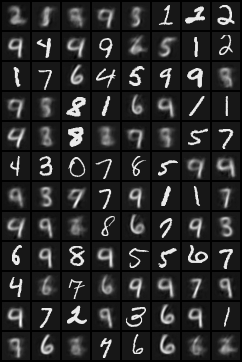
\includegraphics[width=0.6\columnwidth]{{images/mnist_adver_input_10.png}}}
    \caption{Mini-batch of samples drawn from the combined data sets of MNIST and generated by our VAE trained on MNIST.}
    \label{fig:adver_disinput}
\end{figure}

In our architecture, the discriminator input is the joined data sets of 
MNIST and the output of our VAE. 
Figure \ref{fig:adver_disinput} shows a typical input for the discriminator.
Here, we can quickly identify the VAE-generated images as the blurrier ones.
The task is thus too simple, and we would need to train the VAE with
the GAN penalty for better results.

As our hybrid architecture is compatible with the CAN architecture proposed by \cite{elgammalCANCreativeAdversarial2017},
and we are interested in combining the two.
The CAN is well-suited to help the VAE create ambiguous examples that would still be
classified as original MNIST images by the classifier.
We would only need to add an ambiguity term to the discriminator's loss as mentioned in \ref{subsec:gan}.

\subsection{Latent Space Exploration for Novelty Search}
\label{subsec:exploration}  

As a part of our objective to investigate the capacities of our VAE in the search for novelty,
we implement the recursive procedure described in section \ref{subsub:latent_expl}.
We generate mini-batches of samples using our VAE trained on MNIST for 40 epochs.

In the first stage, we generate samples through nine iterations of our model
starting from eight random noise input images following the initialisation proposed in \cite{kazakciDigitsThatAre2017}.
Figure \ref{fig:expl_noise} shows the mini-batch of samples that we obtained by applying this procedure.

As a further part of our experimental setup, we then adapt the method by starting from a set of eight images chosen from the Fashion MNIST database. Figure \ref{fig:expl_fashion} illustrates the samples generated with this initialisation. \\

We visually assess that we were not able to reproduce the quality of results 
obtained in \cite{kazakciDigitsThatAre2017}, where new symbols not belonging 
to a class of digits concerning any criteria were obtained.
Using our model, we generated samples belonging exclusively and without 
any ambiguity to known digit classes for both the initialisations that we chose to consider.


\begin{figure}
      \centerline{
        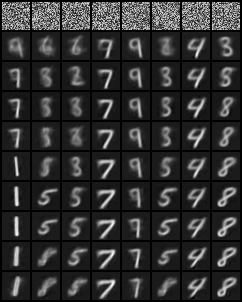
\includegraphics[width=0.6\columnwidth]{{images/mnist_expl_noise_40.png}}
        }
 \caption{Mini-batch of samples generated through nine iterations by our VAE trained on MNIST for 40 epochs and initialized on random noise images.}
 \label{fig:expl_noise}
\end{figure}

\begin{figure}
      \centerline{
        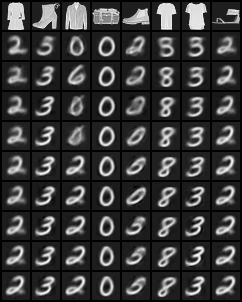
\includegraphics[width=0.6\columnwidth]{{images/mnist_expl_fashion_40.png}}
        }
 \caption{Mini-batch of samples generated through nine iterations by our VAE trained on MNIST for 40 epochs and initialized on images chosen from the Fashion MNIST database.}
 \label{fig:expl_fashion}
\end{figure}


%%%%%%%%%%%%%%%%%%%%%%%%%%%%%%%%%%%%%%%%%%%%%%%%%%%%%%%%%%%%

\section{Conclusions and Perspectives}

At the stage of submitting the results that we have obtained on this project,
we regret that we have not been able to accomplish a fully-working audio VAE.
Thus, some further work on our code would allow us to explore the hereabove
described methods for novelty search in the domain of audio.
\\
From a qualitative point of view, we note the lack of ability to reproduce the results of previous work on creating new symbols by using a VAE trained on MNIST. In this regard, considering models that provide latent spaces of larger dimensions could allow richer explorations and thus tackle the issue of novelty creation, for instance by applying perturbation operations on the latent space representations \cite{kazakciDigitsThatAre2017}.

\section{Contributions}

\begin{itemize}
    \item Zhuomin LIU: MNIST VAE, adversarial VAE; % à remplir
    \item Pierre THIEL: project architecture, MNIST VAE, exploration of latent space, model corruption, adversarial noise;
    \item Christophe WEIS: MNIST VAE, exploration of latent space;
    \item Roy YAKOOB AL HAKEEM: MNIST VAE, model corruption;
\end{itemize}

%%%%%%%%%%%%%%%%%%%%%%%%%%%%%%%%%%%%%%%%%%%%%%%%%%%%%%%%%%%%

%\section{Bibliography}

%\addcontentsline{toc}{section}{ Reference}
%\printbibliography[title={{\it References}}]
%\printbibliography*
%\printbibliography[heading=bibintoc]
\bibliography{ref_am}


%\newpage
%\\
%\newpage

% \subsection{Figures, Tables and Captions}

% All artwork must be centered, neat, clean, and legible.
% All lines should be very dark for purposes of reproduction and art work should not be hand-drawn.
% The proceedings are not in color, and therefore all figures must make sense in black-and-white form.
% Figure and table numbers and captions always appear below the figure.
% Leave 1 line space between the figure or table and the caption.
% Each figure or table is numbered consecutively. Captions should be Times 10pt.
% Place tables/figures in text as close to the reference as possible.
% References to tables and figures should be capitalized, for example:
% see \figref{fig:example} and \tabref{tab:example}.
% Figures and tables may extend across both columns to a maximum width of 17.2cm.

% \begin{table}
% \begin{center}
% \begin{tabular}{|l|l|}
%  \hline
%  String value & Numeric value \\
%  \hline
%  Hello ISMIR  & \conferenceyear \\
%  \hline
% \end{tabular}
% \end{center}
% \caption{Table captions should be placed below the table.}
% \label{tab:example}
% \end{table}

% \begin{figure}
% \centerline{\framebox{
% \includegraphics[width=0.9\columnwidth]{figure.png}}}
% \caption{Figure captions should be placed below the figure.}
% \label{fig:example}
% \end{figure}






%\section{Equations}

%Equations should be placed on separate lines and numbered.
%The number should be on the right side, in parentheses, as in \eqnref{relativity}.

%\begin{equation}\label{relativity}
%E=mc^{2}
%\end{equation}

%All bibliographical references should be listed at the end of the submission, in a section named ``REFERENCES,''
%numbered and in the order that they first appear in the text. Formatting in the REFERENCES section must conform to the
%IEEE standard (\url{https://ieeeauthorcenter.ieee.org/wp-content/uploads/IEEE-Reference-Guide.pdf}). Approved
%IEEE abbreviations (Proceedings $\rightarrow$ Proc.) may be used to shorten reference listings. All references listed
%should be cited in the text. When referring to documents, place the numbers in square brackets (e.g., \cite{ISMIR17Author:01}
%for a single reference, or \cite{JNMR10Someone:01,Book20Person:01,Chapter09Person:01} for a range).

%\textcolor{red}{As submission is double blind, refer to your own published work in the third person. That is, use ``In the previous work of \cite{ISMIR17Author:01},'' not ``In our previous work \cite{ISMIR17Author:01}.'' If you cite your other papers that are not widely available (e.g., a journal paper under review), use anonymous author names in the citation, e.g., an author of the form ``A. Anonymous.''}

\end{document}

